\subsection{Digital ATCO Assistant}

While \gls{AI} has introduced numerous benefits in \gls{ATM}, the current interfaces for \gls{ATC} remain largely passive, limited to information provision. 
Decision-making and high-cognitive-load tasks still rely heavily on human \glspl{ATCO}. 
To meet the increasing demands of global air traffic, a shift toward higher automation levels in \gls{ATC} systems is essential. 
This transition requires a redefinition of task distribution between human controllers and \gls{AI}-based assistants.

Jameel et al. \cite{Jameel_2023} propose a digital \gls{ATCO} architecture combined with a \gls{HAT} interface, forming key components of a highly automated \gls{CWP} for en-route traffic. 
The digital \gls{ATCO} is designed to handle time-intensive tasks such as conflict detection and resolution, generating advisories and commands, and communicating with pilots. 
This enables human \glspl{ATCO} to adopt a supervisory role, potentially reducing the requirement from two to one human controller per sector.

The \gls{HAT} interface plays a central role by providing an intuitive interaction mechanism between human operators and \gls{AI} systems. 
It supports three modes of control: human, hybrid, and autonomous, ensuring flexibility and maintaining human oversight.

\begin{figure}[!ht]
    \centering
    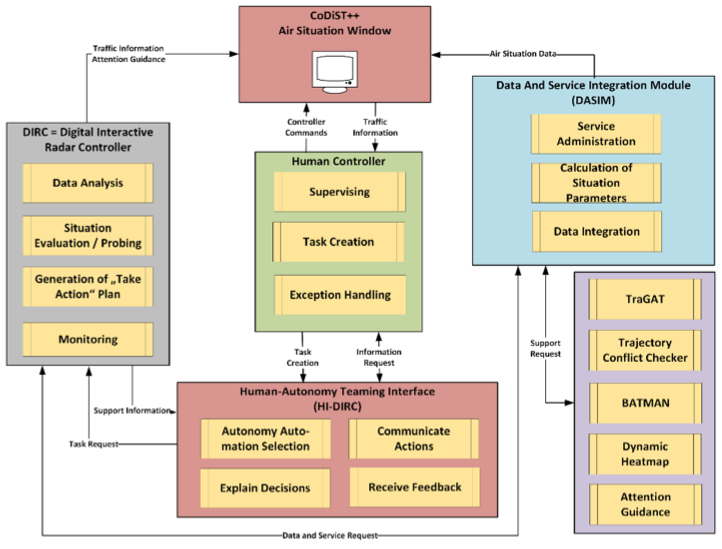
\includegraphics[width=.7\textwidth]{img/digital-atco.png}
    \caption{Overview of the system that enables single human \gls{ATCO} assisted by a digital \gls{ATCO}. \cite{Jameel_2023}}
    \label{digital-atco}
\end{figure}

Figure \ref{digital-atco} illustrates the architecture, which consists of the following core components:
\begin{enumerate}
    \item \gls{CoDiST}: a radar display system supporting primary \gls{ATCO} tasks.
    \item \gls{DIRC}: the digital \gls{ATCO} responsible for traffic control, action planning, and execution.
    \item \gls{HAT} Interface (HI-DIRC): the \gls{HAT} interface enabling communication between human and digital \glspl{ATCO}.
    \item \gls{DASIM}: a data integration system ensuring seamless information access.
    \item Various support tools including:
        \begin{itemize}
            \item \gls{TraGAT}: for generating optimised flight trajectories.
            \item \gls{TCC}: for continuous trajectory conflict checks.
            \item \gls{BATMAN}: for coordination and handover readiness.
            \item \gls{DHM}: for detecting sector congestion and hotspots.
            \item \gls{AG}: for highlighting critical flight events on the radar.
        \end{itemize}
\end{enumerate}

A proof-of-concept \gls{CWP} was showcased at Airspace World 2023, where it received positive feedback. 
Professional \glspl{ATCO} expressed particular interest in shaping further development and validation of the system.

Looking ahead, future research will focus on task allocation strategies to maximise efficiency gains from automation while ensuring operational safety. 
This includes identifying which tasks provide the highest benefit when delegated to \gls{AI}, refining human-in-the-loop control strategies, and ensuring seamless reallocation of tasks from digital \gls{ATCO} back to humans under uncertainty or failure conditions. 
Emphasis will also be placed on increasing the transparency and explainability of \gls{AI} decision-making to build trust and support certification for operational deployment.


% Despite benefits of \gls{AI} use in \gls{ATM} are being observed, the interface for managing air traffic is still limited passively to provdiing information, leaving the bulk of the tasks for human controllers, especially tasks involving decision making.
% To meet the growing demands of air traffic, one way is to increase the level of automation in \gls{ATC} systems. 
% This requires a completely new task distribution for human controllers in combination with \gls{AI}-based systems.

% Jameel et al \cite{Jameel_2023} have designed a digital \gls{ATCO} and the \gls{HAT} interface as two crucial components of highly automated \gls{CWP} for en-route traffic.
% The digital \gls{ATCO} is designed with the capabilities to perform several time-consuming tasks, including conflict detection, conflict resolution, advisories, command creation and the ability to communicate with pilots using CPDLC. 
% It allows the human \gls{ATCO} to take on a more supervisory role, and also reduce the requirement of two human \glspl{ATCO} to just one for managing en-route traffic. 
% The \gls{HAT} interface is the enabling compoennt for a higher automated system as it provides interaction mechanics between human and \gls{AI} systems. 
% The \gls{HAT} interface design also gives human supervisory control over digital \gls{ATCO} operations, with three control modes: human, hybrid, and autonomous.

% This digital \gls{ATCO} architecture system is presented in Figure \ref{}.
% The main components of the systems are:
% \begin{enumerate}
%     \item \Gls{CoDiST}: a human \gls{ATCO} radar display able to perform primary \gls{ATCO} tasks
%     \item \Gls{DIRC}: a digital \gls{ATCO}, capable of handling traffic controller tasks, including generating action plans and implementing them
%     \item \Gls{HI}-\gls{DIRC}: a \gls{HAT} interface with a communication medium between human and digital \gls{ATCO}
%     \item \Gls{DASIM}: to allow seamless information retrieval and access
%     \item Various services and tools automating \gls{ATCO} tasks.
% \end{enumerate}
% These various services includes \gls{TraGAT}, which is able to create optimised trajectories of flights, \gls{TCC} to check trajectories for conflicts on a regular basis, \gls{BATMAN} to provide information and advisories to fulfill the conditions to handover a flight to the next adjacent sector, \glspl{DHM} to highlight the build-up of congestion or hotspots in the \gls{ATCO} area of responsibility and \gls{AG} to highlight flight events on the radar display.

% The proof of concept setup of \gls{CWP} was developed and presented at the Airspace World 2023. 
% The digital \gls{ATCO} concept was appreciated by the participants of the trade show, with actual \glspl{ATCO} especially interested in providing their inputs in the design improvement and validation phases of the projects.

% While this is just a prototype, there are plenty of future works that can be performed on it, such as deligating the task of highest benefit based on its theoretical design, while understanding the limitations of digital \gls{ATCO} and be able to redeligate the process back to human control.




